%   DOCUMENT CLASS  %%%%%%%%%%%%%%%%%%%%%%%%%%%%%%%%%%%%%%%%%%%%%%%%%%%%%%%%%%%
%
%   Use the `sfuthesis` class to format your thesis.
%
%   For more information about thesis formatting requirements, go to http://www.lib.sfu.ca/help/publish/thesis or ask a thesis advisor at the SFU Research Commons.


\documentclass{sfuthesis}



%   DOCUMENT METADATA  %%%%%%%%%%%%%%%%%%%%%%%%%%%%%%%%%%%%%%%%%%%%%%%%%%%%%%%%
%
%   Fill in the following information for the title page and declaration of committee page. Please review the Declaration of Committee page instructions on the library's thesis website before completing this page: https://www.lib.sfu.ca/help/publish/thesis/format/declaration-committee

% Choose the \faculty entry below from the following list:
% Faculty of Applied Sciences
% Faculty of Arts and Social Sciences
% Beedie School of Business
% Faculty of Communication, Art and Technology
% Faculty of Education
% Faculty of Environment
% Faculty of Health Sciences
% Faculty of Science

\title{An example of a thesis on puppies}
\thesistype{Thesis}
\author{H. P. Lovecraft}
\previousdegrees{blag}
\degree{Basketry}
\department{Applied necromancy}
\faculty{Faculty of Example Names}
\copyrightyear{2021}
\semester{Fall 2021}


%You may include up to six keywords or phrases. Keywords should be separated with semicolons. No punctuation at the end.
\keywords{thesis template; Simon Fraser University; \LaTeX; time travel paradoxes}

\committee{
	\chair{Pamela Isely}{Assistant Professor, Computing Science}
	\member{Emmett Brown}{Supervisor \\ Professor, Computing Science}
	\member{Bonnibel Bubblegum}{Committee Member \\ Associate Professor, Computing Science}
	\member{James Moriarty}{Committee Member \\ Adjunct Professor, Computing Science}
	\member{Kaylee Frye}{Examiner \\ Assistant Professor, Engineering Science}
	\member{Hubert J.\ Farnsworth}{External Examiner \\ Professor \\ Department of Quantum Fields \\ Mars University}
}



%   PACKAGES %%%%%%%%%%%%%%%%%%%%%%%%%%%%%%%%%%%%%%%%%%%%%%%%%%%%%%%%%%%%%%%%%%
%
%   Add any packages you need for your thesis here.
%   You don't need to call the following packages, which are already called in
%   the sfuthesis class file:
%
%   - appendix
%   - etoolbox
%   - fontenc
%   - geometry
%   - lmodern
%   - nowidow
%   - setspace
%   - tocloft
%
%   If you call one of the above packages (or one of their dependencies) with
%   options, you may get a "Option clash" LaTeX error. If you get this error,
%   you can fix it by removing your copy of \usepackage and passing the options
%   you need by adding
%
%       \PassOptionsToPackage{<options>}{<package>}
%
%   before \documentclass{sfuthesis}.
%
%   The following packages are a few suggestions you might find useful.
%
%   (1) amsmath and amssymb are essential if you have math in your thesis;
%       they provide useful commands like ``blackboard bold'' symbols and
%       environments for aligning equations.
%   (2) amsthm includes allows you to easily change the style and numbering of
%       theorems. It also provides an environment for proofs.
%   (3) graphicx allows you to add images with \includegraphics{filename}.
%   (4) hyperref turns your citations and cross-references into clickable
%       links, and adds metadata to the compiled PDF.
%   (5) pdfpages lets you import pages of external PDFs using the command
%       \includepdf{filename}. You will need to do this if your research
%       requires an Ethics Statement.
%

\usepackage{amsmath}                            % (1)
\usepackage{amssymb}                            % (1)
\usepackage{amsthm}                             % (2)
\usepackage{graphicx}                           % (3)
\usepackage[pdfborder={0 0 0}]{hyperref}        % (4)
% \usepackage{pdfpages}                         % (5)
% ...
% ...
% ...
% ... add your own packages here!

\usepackage{longtable}


%   OTHER CUSTOMIZATIONS %%%%%%%%%%%%%%%%%%%%%%%%%%%%%%%%%%%%%%%%%%%%%%%%%%%%%%
%
%   Add any packages you need for your thesis here. We've started you off with
%   a few suggestions.
%
%   (1) Use a single word space between sentences. If you disable this, you
%       will have to manually control spacing around abbreviations.
%   (2) Correct the capitalization of "Chapter" and "Section" if you use the
%       \autoref macro from the `hyperref` package.
%   (3) The LaTeX thesis template defaults to one-and-a-half line spacing. If
%       your supervisor prefers double-spacing, you can redefine the
%       \defaultspacing command.
%

\frenchspacing                                    % (1)
\renewcommand*{\chapterautorefname}{Chapter}      % (2)
\renewcommand*{\sectionautorefname}{Section}      % (2)
\renewcommand*{\subsectionautorefname}{Section}   % (2)
% \renewcommand{\defaultspacing}{\doublespacing}  % (3)
% ...
% ...
% ...
% ... add your own customizations here!

\providecommand{\tightlist}{%
  \setlength{\itemsep}{0pt}\setlength{\parskip}{0pt}}

%   FRONTMATTER  %%%%%%%%%%%%%%%%%%%%%%%%%%%%%%%%%%%%%%%%%%%%%%%%%%%%%%%%%%%%%%
%
%   Title page, committee page, abstract, dedication, acknowledgements, table of contents, etc.
%
%   If your research requires an Ethics Statement, download one from the SFU library website at https://www.lib.sfu.ca/help/publish/thesis/regulations#ethics-statement, save the relevant pdf to your thesis folder, and then uncomment the appropriate lines below.

\begin{document}

\frontmatter
\maketitle{}
\makecommittee{}

%\addtoToC{Ethics Statement}%
%\includepdf[pagecommand={\thispagestyle{plain}}]{ethics_statement_piii.pdf}%
%\clearpage

\begin{abstract}
Abstract paragraphs should be unindented. Master's abstracts are limited to 150 words; the limit is 350 words for doctoral abstracts. Abstract text must fit on a single page.
\end{abstract}


\begin{dedication}
This is an optional page. Use your choice of paragraph style for text on this page. \end{dedication}


\begin{acknowledgements}
This is an optional page. Use your choice of paragraph style for text on this page. \end{acknowledgements}

\addtoToC{Table of Contents}%
\tableofcontents%
\clearpage

%This is an optional page. Remove the following lines if you don't have any tables.
\addtoToC{List of Tables}%
\listoftables
\clearpage

%This is an optional page. Remove the following lines if you don't have any figures.
\addtoToC{List of Figures}%
\listoffigures
\clearpage





%   MAIN MATTER  %%%%%%%%%%%%%%%%%%%%%%%%%%%%%%%%%%%%%%%%%%%%%%%%%%%%%%%%%%%%%%
%
%   Start writing your thesis --- or start \include ing chapters --- here.
%

\mainmatter%

\hypertarget{introduction}{%
\section*{Introduction}\label{introduction}}
\addcontentsline{toc}{section}{Introduction}

Welcome to the \emph{R Markdown} thesis template. This template is based on (and in many places copied directly from) the Reed College LaTeX template, but hopefully it will provide a nicer interface for those that have never used TeX or LaTeX before. Using \emph{R Markdown} will also allow you to easily keep track of your analyses in \textbf{R} chunks of code, with the resulting plots and output included as well. The hope is this \emph{R Markdown} template gets you in the habit of doing reproducible research, which benefits you long-term as a researcher, but also will greatly help anyone that is trying to reproduce or build onto your results down the road.

Hopefully, you won't have much of a learning period to go through and you will reap the benefits of a nicely formatted thesis. The use of LaTeX in combination with \emph{Markdown} is more consistent than the output of a word processor, much less prone to corruption or crashing, and the resulting file is smaller than a Word file. While you may have never had problems using Word in the past, your thesis is likely going to be about twice as large and complex as anything you've written before, taxing Word's capabilities. After working with \emph{Markdown} and \textbf{R} together for a few weeks, we are confident this will be your reporting style of choice going forward.

\textbf{Why use it?}

\emph{R Markdown} creates a simple and straightforward way to interface with the beauty of LaTeX. Packages have been written in \textbf{R} to work directly with LaTeX to produce nicely formatting tables and paragraphs. In addition to creating a user friendly interface to LaTeX, \emph{R Markdown} also allows you to read in your data, to analyze it and to visualize it using \textbf{R} functions, and also to provide the documentation and commentary on the results of your project. Further, it allows for \textbf{R} results to be passed inline to the commentary of your results. You'll see more on this later.

\textbf{Who should use it?}

Anyone who needs to use data analysis, math, tables, a lot of figures, complex cross-references, or who just cares about the final appearance of their document should use \emph{R Markdown}. Of particular use should be anyone in the sciences, but the user-friendly nature of \emph{Markdown} and its ability to keep track of and easily include figures, automatically generate a table of contents, index, references, table of figures, etc. should make it of great benefit to nearly anyone writing a thesis project.

\textbf{For additional help with bookdown}

Please visit \href{https://bookdown.org/yihui/bookdown/}{the free online bookdown reference guide}.

\hypertarget{abstract}{%
\section{Abstract}\label{abstract}}

Effective wildlife conservation often requires understanding diet composition and its consequences for population demographics. We measured breeding season diet of an at-risk population of northern goshawks (\emph{Accipiter gentilis}) in coastal British Columbia using a combination of egested pellets, prey remains, and nest camera photos. We compared diet composition across two ecological zones and assessed the impact of diet diversity and dietary specialization on goshawk productivity. Our results differed between source (pellets, remains, or cameras) and measurement (biomass or counts), highlighting the importance of clearly reporting methods in raptor diet studies. Goshawks consumed 29 different prey species but primarily consumed tree squirrels (\emph{Tamiascuirus} spp.), with this single taxon making up 59\% of the biomass delivered to nests. Diet composition differed slightly between ecological zones but dietary specialization on tree squirrels was equally high in both zones. Goshawk nests monitored with nest cameras fledged 1.4 \(\pm\) 0.79 chicks. However, we found no evidence to support an effect of diet diversity or dietary specialization on variation on goshawk productivity.

\hypertarget{general-introduction}{%
\section{General Introduction}\label{general-introduction}}

Once valued primarily for high timber yields, temperate rainforests of the Pacific Northwest are now managed with increased emphasis on the conservation of biodiversity (Thomas et al. 2006). Among the drivers of this shift are declining populations of species whose life histories depend on old-growth forests. Some of these species have been placed under federal, provincial, or state protection: among others, the marbled murrelet (\emph{Brachyramphus marmoratus}) is protected under the Species at Risk Act in Canada (COSEWIC 2014) and the coastal population of the pacific marten (\emph{Martes caurina}) is protected under the Endangered Species Act in the United States (Wildlife Service 2020). Management under these types of legislation is typically reactive and focuses on conserving each imperiled species on a case-by-case basis (Simberloff 1998). This approach has been widely criticized for failing to provide management for wider ecosystems, including the very ecosystems on which the imperiled species depend (Lambeck 1997). Alternatively, focusing on the broader scales of landscapes or ecosystems should preserve the ecosystem processes and services on which wild species and humans alike depend (Franklin 1993 ). Yet ecosystem-based management is itself beset by numerous practical, theoretical, and even philosophical challenges which have made it difficult to implement (Lambeck 1997, Simberloff 1998).

Managers have often turned to surrogate species as a solution for the dilemma posed by the single-species and ecosystem-based management debate. At the core of the surrogate species concept is the belief that the requirements or wellbeing of a single species, or a small suite of species, can stand in for the needs and health of numerous co-occurring species or entire ecosystems (Caro 2010). Numerous variations and conflicting definitions are present in the literature, but the original concept may be that of the \emph{indicator species}. The presence and population size of an indicator species is believed to reflect ecosystem processes or the populations of other species (Landres et al.~1988). Perhaps more widespread than indicator species is the \emph{umbrella species} concept. Protections which benefit umbrella species--typically wide-ranging habitat specialists--are assumed to confer protection to co-occurring species with smaller ranges and less restrictive habitat requirements (Roberge \& Angelstam 2004, Seddon \& Leech 2008). A related concept is the \emph{flagship species}, a species whose protection, like an umbrella species, confers benefit on other species, but which is selected for its charisma and ability to serve as a rallying point for conservation (Andelman \& Fagan 2000). These concepts all attempt to extend the relative simplicity of single-species methods to achieve the promise of ecosystem-based management (Lambeck 1997).

No species better embodies the challenges of managing forest species and ecosystems in the Pacific Northwest than the northern spotted owl (\emph{Strix occidentalis caurina}). The spotted owl is strongly associated with old-growth temperate rainforests (Forsman et al. 2004) and has at various points been proposed as an indicator (Gutiérrez and Carey 1985), an umbrella (Tracy and Brussard 1994), and a flagship species for this ecosystem. In the late 1980s, public outcry and litigation in the United States led to the development of a spotted owl conservation strategy concurrent with the species' listing as threatened under the Endangered Species Act (Thomas et al. 2006). This single-species plan rapidly expanded to include other species, particularly the marbled murrelet and several salmon stocks, and ultimately evolved into the Northwest Forest Plan. The Northwest Forest Plan remained rooted in spotted owl management, but also included protections for watersheds, monitoring of rare species, and a sustainable annual timber harvest (DellaSala and Williams 2006). Not all the Northwest Forest Plan's goals have been achieved--notably, spotted owl and marbled murrelet populations have continued to decline, although at a slower rate--and some parts of the plan have been eroded under subsequent presidential administrations (DellaSala et al. 2015). Yet the Northwest Forest Plan remains a powerful example of an ecosystem-based management plan with a single species at its core.

The story of the northern goshawk (\emph{Accipiter gentilis}) in North America parallels that of the spotted owl. Goshawks are found in boreal forests across the continent and range as far south as the high-elevation forests of the American Southwest. Two subspecies (\emph{A. g. atricapillus} and \emph{A. g. laingi}) are widely recognized and a third (\emph{A. g. apache}) is acknowledged by some authors (Squires et al. 2020). Goshawks are not associated with old-growth forest to the same degree as the spotted owl, but do show a clear preference for extensive tracts of mature forest with large-diameter trees and closed canopies (Andersen et al. 2005, Squires and Kennedy 2006). Like the spotted owl, goshawks have been proposed as a flagship (Sergio et al. 2006), an indicator, and an umbrella species (Ozaki et al. 2006). In the American Southwest, alarms were sounded over the impact of timber harvest on northern goshawks at the same time the Northwest Forest Plan was developing in the Pacific Northwest (Crocker-Bedford 1990). Decades of litigation failed to result in listing the southwestern population (proposed subspecies \emph{apache}) under the Endangered Species Act, but a new management plan was eventually developed (Peck 2000). This single-species management plan disallowed timber harvest near known goshawk nests and required a minimum amount of mature forest within the larger home range surrounding nests (Reynolds et al. 1992). Notably, the plan also specified the inclusion of younger forest, small clearings, snags, and woody debris to provide habitat for eight important goshawk prey species. This recommendation was based on the assumption that goshawks are habitat generalists limited by the abundance, not the availability, of prey--an assumption which has been the subject of heated debate (Greenwald et al. 2005, Reynolds et al. 2008). However, by incorporating multiple species, dynamic ecosystem processes, and human use, the goshawk management plan approaches the principles of ecosystem-based management and shows its potential to scale up to a more cohesive plan in the style of the Northwest Forest Plan (Graham et al. 1994, Peck 2000).

In the Pacific Northwest, naturalists described a small, dark subspecies of goshawk unique to the coastal temperate rainforests of Haida Gwaii and Vancouver Island (Taverner 1940). The size and plumage characteristics of \emph{A. g. laingi} may be an adaptation the dark, dense forests the subspecies inhabits (Ethier 1999) and the agile avian prey believed to dominate its diet (Penteriani et al. 2013, McClaren et al. 2015). The precise range of \emph{laingi} is unclear; based on morphometrics, genetics, and ecosystem mapping, it is believed to extend along the west coast and islands of British Columbia, from Southeast Alaska south to Washington's Olympic Peninsula (Team 2008, Sonsthagen et al. 2012). In the portion of its range within the United States the \emph{laingi} subspecies has no additional protections, but in Canada it is designated as Threatened by the Committee on the Status of Endangered Wildlife in Canada (COSEWIC). The \emph{laingi} subspecies is further Red-listed by the British Columbia Conservation Data Centre and is an Identified Wildlife Species under the Forest Practices Code (COSEWIC 2013). Existing management plans call for the creation of buffers around known goshawk nests and the maintenance of a minimum amount of mature forest within the larger home range, similar to the plan from the American Southwest (McClaren et al. 2015, Agency 2018). However, plans do not include recommendations for providing habitat for goshawk prey species. To some extent this is due to the single-species nature of the plan, but it is also a result of several knowledge gaps. Goshawk managers have acknowledged that a landscape-scale plan would be superior to the current fine-scale plan, and ecosystem-based management has been implemented elsewhere in British Columbia, most notably the Great Bear Rainforest (Price et al. 2009 ). Together these suggest an ecosystem-based approach incorporating the goshawk as a focal species may be possible for coastal rainforests elsewhere in British Columbia. Yet while \emph{laingi} nesting habitat is relatively well documented, foraging behavior and habitat remain poorly understood. The knowledge gaps surrounding goshawk foraging ecology hinder current single-species and potential ecosystem-based management alike.

My thesis attempts to fill one knowledge gap identified by the Northern Goshawk Recovery Team (NGRT) by providing basic ecological information regarding the breeding season diet of goshawks in coastal British Columbia (Team 2008). The following chapter describes my research quantifying goshawk diet in coastal British Columbia and investigating potential links between dietary variation and goshawk reproductive success. The final chapter summarizes my results, describes the outcome of a pilot study of goshawk space-use, and discusses the implications of both for management and future research efforts.

\hypertarget{general-conclusion}{%
\section{General Conclusion}\label{general-conclusion}}

\hypertarget{overview}{%
\subsection{Overview}\label{overview}}

Specialist and generalist predators differ in their degree of dependence on prey species with cascading consequences for many aspects of their life history (Korpimaki and Norrdahl 1991, Resano‐Mayor et al. 2016). Specialist predators are efficient hunters of their main prey at the cost of poor success when hunting other species, whereas generalist predators hunt many species with equal skill (Terraube et al. 2011). A specialist predator may struggle to compensate when its main prey becomes scarce, but generalist predators readily switch to alternate prey (Steenhof and Kochert 1988, Terraube and Arroyo 2011). As a result, specialist predators depend on a single species and their demographic parameters--such as migration, reproductive success, and survival--vary in synchrony with its abundance (Korpimaki and Norrdahl 1991, Terraube et al. 2011). In contrast, generalist predators make use of many species and their populations are relatively stable (Andersson and Erlinge 1977, Hanski et al. 1991).

The familiar dichotomy between specialist and generalist predators is, of course, an oversimplification. The abundance of a single prey species can be a major driver of demographic parameters, such as reproductive success, for a generalist and specialist predators alike (Elmhagen et al. 2000, Resano‐Mayor et al. 2016). Furthermore, within a single species some populations (Salamolard et al. 2000, Roth et al. 2007), or some individuals within a population (Woo et al. 2008), may be more or less specialized. A single individual may also become more specialized over its lifetime as a result of age and experience (Rutz 2006). Correctly identifying the degree of specialization and understanding its effect on demographic parameters is more than a matter of theory or curiosity: the consequences of specialization can scale up from individuals through populations to entire species, with profound implications for conservation (Ferrer and Negro 2004, Terraube et al. 2011, Resano‐Mayor et al. 2016).

The complex relationship between dietary specialization and conservation is exemplified by the northern spotted owl (\emph{Strix occidentalis caurina}). Spotted owls depend on old-growth forests, but the cause of this association has been a source of speculation from the earliest years of spotted owl research (Gutiérrez and Carey 1985). The association appears to be driven, in part, by the spotted owl's relatively specialized diet (Carey et al. 1992, Ward et al. 1998). More than half the biomass spotted owls consume comes from just two taxa, flying squirrels (\emph{Glaucomys sabrinus}) and woodrats (bushy-tailed woodrat \emph{Neotoma cinerea} and dusky-footed woodrat \emph{N. fuscipes}; reviewed in Carey et al. (1992)). This holds true across the subspecies' range, although the relative contribution of each taxa varies with geographic region and forest type in response to local abundance. In Washington's Olympic Peninsula, where woodrats are absent, spotted owls consume primarily flying squirrels (Carey et al. 1992), whereas in northern California flying squirrels make up a smaller portion of the diet and woodrats, which are more abundant, dominate (Ward et al. 1998). Even within a single spotted owl population some individuals specialize on one taxa or the other (Zabel et al. 1995). Home range sizes in the flying squirrel-dependent Olympic Peninsula are among the largest ever recorded (Carey et al. 1992), and where both taxa are present owls which consume primarily flying squirrels have larger home ranges than those which consume mostly woodrats (Zabel et al. 1995). Evidently diet and prey abundance affect some demographic parameters, such as breeding density, which has led some authors to recommend increasing prey abundance as a route to increase owl abundance (Forsman et al. 2004). Yet prey abundance does not appear to affect spotted owl productivity (Rosenberg et al. 2003). Instead, productivity appears to be the result of complex interactions between climate and prey abundance (Glenn et al. 2011).

In contrast to the spotted owl's dependence on a few prey species, the northern goshawk is considered a generalist predator and consumes an enormous diversity of prey across its wide geographic range (reviewed in Drennan 2006, Rutz et al. 2006). I identified 29 different prey species in the diet of goshawks in coastal British Columbia, which is consistent with a generalist foraging strategy. However, over 60\% of goshawk diet in my study area was composed of tree squirrels (\emph{Tamiasciurus} spp.), which indicates a level of specialization even greater than that of the spotted owl. Some goshawk populations appear to be strongly generalist (e.g.~Arizona, Salafsky et al. 2007), whereas in others a key prey species is a major driver of productivity, survival, and other demographic parameters (e.g.~Yukon, Doyle and Smith 1994, and Finland, Tornberg et al. 2005). I found no affect of the degree of dietary specialization on goshawk productivity. There are several explanations for this unexpected finding. First, specialists may not be more productive than generalists. Specialist individuals may preferentially consume tree squirrels but have similar levels of fitness as generalist individuals in this population (Woo et al. 2008). Alternately, specialization may not be the result of preference. Individuals may lack strong prey preferences and take tree squirrel in proportion to their abundance. Total prey abundance, rather than tree squirrel abundance, may drive productivity (Salafsky et al. 2007 ). Finally, as in the spotted owl, prey abundance and diet during the breeding season may be a lesser driver of productivity than other factors, such as weather or winter prey abundance.

Goshawk diet varies across its range in response to the regional presence and abundance of prey species (Drennan 2006). I found the key prey of goshawks in the south coast region was tree squirrels. This contrasts with studies of goshawk diet elsewhere in the Pacific Northwest where the key prey is generally grouse (Watson et al. 1998, Thrailkill et al. 2000, Bloxton 2002, Lewis et al. 2006), but is similar to work on Vancouver Island where the key prey is also tree squirrels (Ethier 1999). My results also contrast with studies from other regions of western North America where the key prey may occasionally be a species of squirrel, but is most often a species of hare or rabbit. The unexpected difference between diet in my study area and the larger Pacific Northwest may in part be due to differences in methodology. When the results from studies across temperate rainforest ecosystems are standardized (data from pooled pellets-and-remains or remains only, measured by counts), the contrast between regions within the Pacific Northwest is much less pronounced. However, the proportion of mammalian prey, particularly tree squirrels, in the diet remains markedly higher within coastal British Columbia than outside it. Tree squirrel abundance is higher in the south coast region than in other temperate rainforest ecosystems (Carey 1995, Ransome and Sullivan 2003). No Pacific Northwest study has assessed goshawk diet and and absolute prey abundance simultaneously (but see Ethier (1999)). Nonetheless, regional data hint at a pattern of higher dietary specialization in regions or forest types with higher tree squirrel abundance (see Figure \ref{fig:squirrel-map}). Across the two ecological zones present in my study area I observed only minor variation in goshawk diet and no variation in the dominance of tree squirrels in the diet. If goshawks are more specialized on tree squirrels where tree squirrels are more abundant, this would indicate a slight difference in the prey community of these two zones but a similar abundance of tree squirrels. Overall, goshawks in my study area appear to be a generalist predator opportunistically exploiting a locally abundant prey species.

\hypertarget{directions-for-future-research}{%
\subsection{Directions for future research}\label{directions-for-future-research}}

Comparing the foraging ecology of the northern spotted owl and the northern goshawk highlights significant knowledge gaps regarding goshawk biology. The controversy surrounding spotted owl conservation, combined with its position at the heart of a major management plan, has made it one of the most-studied birds in the world (Gutiérrez et al. 2020). The northern goshawk, although likewise shrouded in controversy, has not received the same level of study. Where data are available, it is more difficult to generalize research on the widespread, generalist northern goshawk than for the more restricted, relatively specialized spotted owl. As a result, there is a pressing need for detailed, local information on goshawks in the Pacific Northwest, particularly in coastal British Columbia.

One knowledge gap related to the work I present here is how variation in prey abundance affects the degree of dietary specialization, productivity, and survival of individual goshawks. Dietary specialization such as goshawks in my study area exhibit may be the result of a preference for the main prey or simply an absence of other options. Data on prey abundance is necessary to understand the mechanism of goshawk specialization and whether it is the result of high selectivity for tree squirrels, high abundance of tree squirrels, or some combination of both. This information could in turn be used to evaluate how changes in key prey abundance and total prey abundance influence goshawk demographic parameters, particularly productivity. Without this knowledge it is impossible to fully understand the factors limiting goshawk populations in coastal British Columbia.

A second knowledge gap is how the amount and type of habitat goshawks use for foraging varies with diet and prey abundance. Goshawk home range size varies across their geographic range and goshawks have been observed foraging in diverse habitat types, leading to ongoing debate over how and why goshawks select habitat (Greenwald et al. 2005, Reynolds et al. 2008). Research on spotted owls indicates that home range size is inversely related to prey abundance and foraging habitat selection varies with the identity of the main prey (Zabel et al. 1995). Variation in goshawk home range size and habitat selection may likewise be explained by diet and prey abundance (Kenward 1982, Penteriani et al. 2013). If so, foraging habitat management could only be conducted with knowledge of goshawk diet and recommendations made for one population could be applied to others only with great caution. Filling this knowledge gap with information specific to coastal British Columbia is vital and has been identified as a priority by goshawk managers (Team 2008, Agency 2018).

To address this crucial knowledge gap, the British Columbia Ministry of Forests, Lands, Natural Resource Operations and Rural Development (FLNRORD) and I conducted a pilot study of foraging habitat use in coastal British Columbia. Between 2018-2020 we tagged and tracked 4 male and 9 female goshawks. Captures were conducted during the early breeding season using a dho-gaza trap with a live great-horned owl (\emph{Bubo virginianus}) as a lure (Bloom et al. 2007). Goshawks were fitted with 14-gram solar-powered GPS-UHF tags (Ecotone Telmetry brand, Harrier model) with an additional VHF tag, attached via backpack-style harness. Tags were programmed to take a location point every 15 minutes and to download data to a base station when within range (approximately 100 m from the station). Base stations were placed beneath or above nests and tags checked for proximity to the station every 15 minutes.

We were able to retrieve data from 10 out of 13 birds, collecting location data from 3 to 73 (mean 37.89 \(\pm\) 26.69 standard deviation) days of the breeding season (20 April - 15 September; Table \ref{tab:telemetry-table}). Tracked birds provided 45 - 2964 location points (mean 837.78 \(\pm\) 923) with an average of 31.03 (\(\pm\) 62.28) locations per bird per day. Over the study period we observed only one probable mortality. I estimated breeding season home ranges and core-use areas using 95\% minimum convex polygons (MCPs) and 50\% MCPs, respectively. The mean breeding season home range was 2008.89 ha but male home ranges were far larger than female home ranges (male mean = 4409.16 \(\pm\) 1408.38, n = 4; female mean = 829.13 \(\pm\) 1816.72, n = 5; \emph{t} = -3.5, df = 7.68, \emph{P} = 0.01). Male core-use areas were also larger than female core-use areas, but not significantly so (male mean = 851.51 \(\pm\) 508.29; female mean = 151.87 \(\pm\) 368.85; \emph{t} = -2.37, df = 5.1, \emph{P} = 0.06). Female home ranges and core-use areas were smaller due to the significantly higher amount of time females spent near the nest (\emph{t} = -3.32, df = 6.9, \emph{P} = 0.01). Males also traveled further from the nest than females. The mean furthest distance from the nest a male traveled was 7.05 (\(\pm\) 1.76) km, while on average females only ventured 2.86 (\(\pm\) 2.02) km from the nest (\emph{t} = -3.32, df = 6.9, \emph{P} = 0.01). As the breeding season progressed, the length of time spent away from the nest increased noticeably for males but less so for females. Home ranges were rarely circular, but rather shaped by geographic constraints such as coastlines or mountains peaks (see Figures \ref{fig:rlk-female} and \ref{fig:rlk-male}). Within home ranges, kernel density estimates show habitat use is not even across a male's territory. Instead, there are clusters of activity around areas which are likely high-quality foraging habitat.

We encountered several challenges over the course of the three-year pilot. First, the location data we obtained were biased toward females. Females are more aggressive near the nest than males and so are more likely to be captured when using the dho-gaza trapping method. Data from female tags downloaded more frequently onto the base stations than data from male tags because of the large amount of time females spent near the nest, where the base stations were located. Consequently, we collected far more location data on females than males, which offered relatively little insight into foraging habitat use since males provide most of the food during the breeding season. Second, we were unable to retrieve data from some tagged birds. Several birds were detected via the VHF transmitter but could not be relocated with sufficient precision to download data from the UHF tag. As a result, we could not retrieve data from the winter or subsequent breeding season. Our inability to relocate birds is likely due to a combination of the limited range of the VHF tags and the difficult topography of our study area, compounded by the birds' failure to return to known breeding areas. Finally, technical malfunctions resulted in no data downloads for two birds, too many location points for one birds, and too few location points for many others. Future work should consider more powerful VHF tags for easier relocation and an alternate-days duty cycle to reduce the number of missed locations.

Despite these setbacks, the pilot study provided insight into goshawk movement and habitat use, with relevance to goshawk management. The location data we were able to retrieve, although less than anticipated, was of much higher resolution than VHF data and much higher accuracy than satellite data and may therefore be uniquely well-suited to studies of foraging habitat selection. The high fidelity of females to the nest area confirms the importance of protected buffers around nests to prevent the disturbance of habitat critical for breeding females and fledglings. However, the large distances traveled by males and the irregular shape of their home ranges shows that circular buffers based on estimates of mean home range size are not good approximations of true space use. Areas used extensively by males usually fall outside the nest area and are not be captured by current nesting habitat protections. Preliminary inspection of movement data indicates goshawks readily crossed narrow barriers such as roads, rivers, and powerline cuts, and sometimes appeared to use these features for travel or foraging. On the other hand, goshawks seemed to generally route around larger barriers such as lakes or clearcuts. This suggests managed areas around nests should be tailored to the amount and configuration of suitable foraging habitat present in the surrounding landscape, and that any timber harvest within the foraging area should prioritize the preservation of connectivity between patches of high-quality foraging habitat. However, a great deal of additional research is needed to confirm and refine these suggestions, particularly regarding the characteristics of suitable and high-quality foraging habitat.

\hypertarget{management-implications-of-goshawk-diet}{%
\subsection{Management implications of goshawk diet}\label{management-implications-of-goshawk-diet}}

Climate change is one of the largest and most difficult to anticipate threats facing biodiversity (Bellard et al.~2012). The current understanding of how climate change will impact goshawks in coastal British Columbia is largely speculative (Agency 2018). Although I found no evidence of a link between the degree of dietary specialization and goshawk productivity, the level of specialization I observed and findings from other studies suggest goshawks in my study area are highly dependent on tree squirrels for successful reproduction. Notably, Ethier (1999) found goshawk productivity on Vancouver Island to be significantly correlated with red squirrel abundance. Tree squirrels are themselves highly dependent on conifer seeds and their abundance varies with the size of the annual cone crop (Smith 1970). Seed production is cyclical, but may be increased by higher temperatures and inhibited by drought (Boucher et al. 2020). As the climate warms and drought risk rises, climate-driven changes in seed production may cascade upward through prey abundance to impact goshawk populations in coastal British Columbia. Significantly more work is needed to understand the relationship between prey abundance, the buffering ability of alternate prey, and goshawk productivity, but my results provide an important starting point for incorporating climate change into goshawk management.

Wildlife management, whether founded on a single-species or ecosystem-based approach, generally centers around species, subspecies, or unique populations at risk of extinction. My thesis examines a single population of goshawks on the south coast of British Columbia which is currently classified as part of the subspecies \emph{laingi}. The precise range of \emph{laingi} has never been entirely clear, but recent genetic evidence indicates the Haida Gwaii population is highly unique and distinct from other putative \emph{laingi} populations (Geraldes et al. (2018)). My results suggest a strong ecological similarity between goshawks within my study area, Vancouver Island, and Haida Gwaii, where goshawks are also highly dependent on tree squirrels (COSEWIC 2013). The diet of these populations stands in contrast to others in temperate rainforest ecosystems which are currently considered \emph{laingi}, such as the Olympic Peninsula or Southeast Alaska, where goshawks consume mainly birds. Goshawks in coastal British Columbia may therefore be ecologically similar to each other, and ecologically distinct from other populations, regardless of their genetic relationship. The ecological similarity of these populations supports the strategy used by the Northern Goshawk Recovery Team to delineate the boundaries of the \emph{laingi} range, which relies more on ecosystem mapping than genetics (Team 2008).

Rooting management in ecosystems, rather than individual species, has been a success--albeit a conditional one--for forest conservation in the United States. Ecosystem-based management has also been applied in the temperate rainforests of British Columbia. In the early 2000s an ecosystem-based management plan, which includes the northern goshawk as a focal species, was developed for the Great Bear Rainforest on the northern coast of British Columbia (Price et al. 2009). My work provides some of the habitat-specific ecological information needed to broaden existing single-species goshawk management, or even to incorporate goshawks as a focal species in future ecosystem-based management. While it will be years before the success of Great Bear Rainforest agreement can be assessed, the groundbreaking plan offers a glimpse of the future of forest management in British Columbia--and the role northern goshawks may play in it.

\hypertarget{figures}{%
\section{Figures}\label{figures}}

\begin{figure}
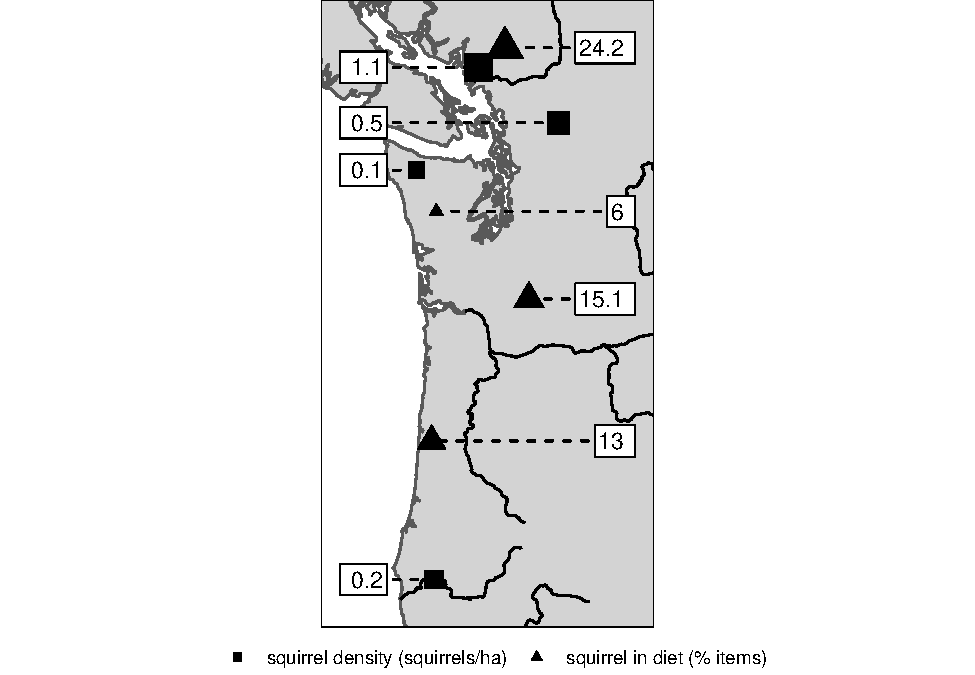
\includegraphics[width=1\linewidth]{index_files/figure-latex/squirrel-map-1} \caption{Comparison of goshawk dietary specialization and squirrel abundance in the Pacific Northwest. Size of symbol represents relative specialization or abundance. Goshawk diet estimated pellets-and-remains or remains only and measured using counts of items. Tree squirrel abundance estimated from number of individuals/ha. Adapted from Carey et al. (1992), Watson et al. (1998), Thrailkill et al. (2000), Bloxton (2002), Ransome and Sullivan (2003), and this study.}\label{fig:squirrel-map}
\end{figure}

\begin{figure}
\centering
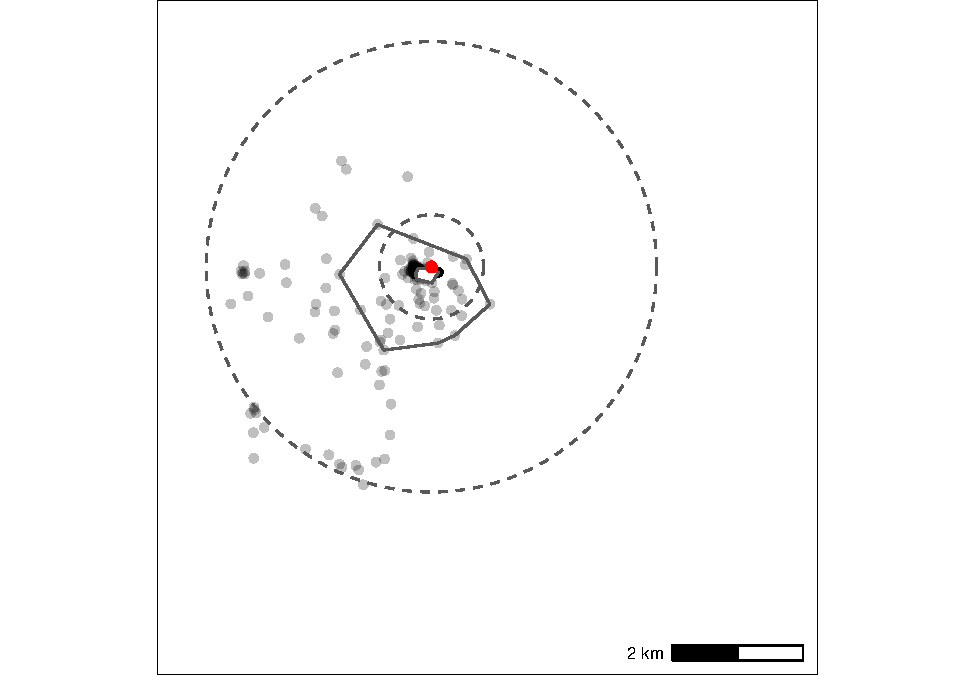
\includegraphics{index_files/figure-latex/rlk-female-1.pdf}
\caption{\label{fig:rlk-female}Breeding season home range and core-use area of one tagged female goshawk in 2020.}
\end{figure}

\begin{figure}
\centering
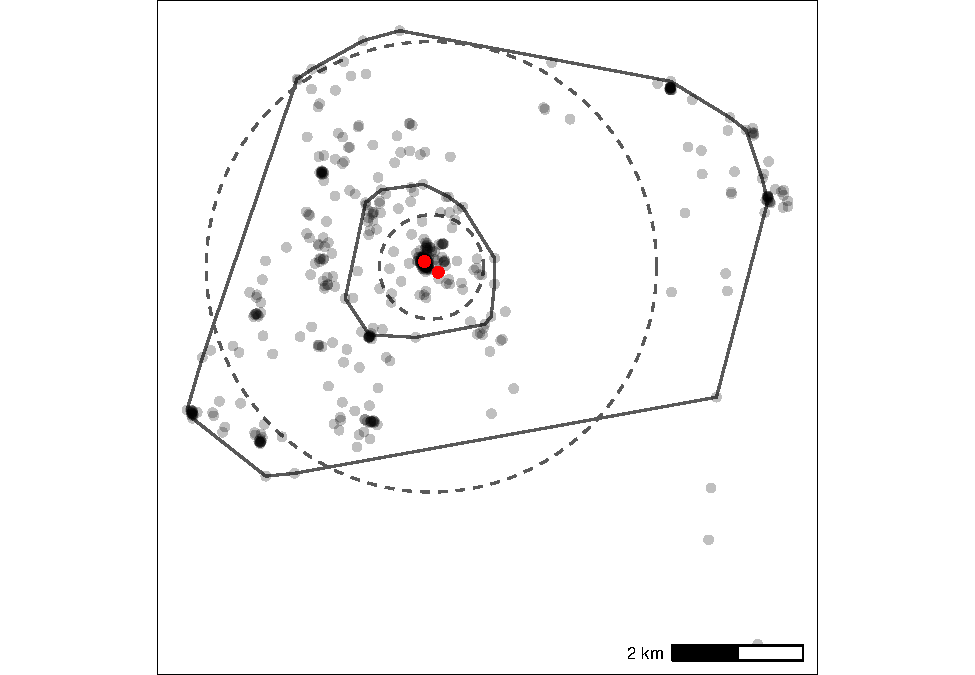
\includegraphics{index_files/figure-latex/rlk-male-1.pdf}
\caption{\label{fig:rlk-male}Breeding season home range and core-use area of one tagged male goshawk in 2019}
\end{figure}

\begin{table}[H]
\centering
\begin{tabular}{l|l|l|l|l|l|l|l|l|l|l|l|l}
\hline
sex & id & site & min & max & period & n.points & dist & prop.at.base & mcp.50 & mcp.95 & kde.50 & kde.95\\
\hline
f & HAR12 & FMT & 2020-06-25 & 2020-06-28 & 3 & 104 & 2.3 & 3.9 & 0.7 & 103.7 & 13 & 152.1\\
\hline
f & HAR03 & GRV & 2020-06-08 & 2020-06-28 & 20 & 2964 & 2.4 & 95.9 & 0 & 0 & 0 & 0\\
\hline
f & HAR10 & MTC & 2019-05-02 & 2019-06-29 & 58 & 315 & 5.5 & 78.4 & 0.3 & 58.9 & 8.7 & 113.4\\
\hline
f & HAR02 & RLK & 2020-06-13 & 2020-07-08 & 25 & 977 & 4 & 72.1 & 5.4 & 280.6 & 12.7 & 267.4\\
\hline
f & HAR08 & TCR & 2019-06-10 & 2019-06-27 & 17 & 45 & 0.1 & 82.2 & 0 & 0.2 & 0 & 0.4\\
\hline
f & AVERAGE & - & - & - & 25 & - & 2.9 & 66.5 & 1.3 & 88.7 & 6.9 & 106.7\\
\hline
m & HAR09 & MTC & 2019-05-02 & 2019-07-02 & 61 & 409 & 4.4 & 2.4 & 530.1 & 2611.2 & 636.3 & 3032.8\\
\hline
m & HAR04 & RLK & 2019-06-22 & 2019-07-08 & 16 & 532 & 7.8 & 9 & 423 & 4441.1 & 662.3 & 4407.6\\
\hline
m & HAR05 & SKA & 2019-06-23 & 2019-09-04 & 73 & 1557 & 8 & 0 & 1548.2 & 6052.9 & 1642.2 & 6674.7\\
\hline
m & HAR07 & TCR & 2018-07-08 & 2018-09-14 & 68 & 637 & 8 & 0 & 904.8 & 4531.4 & 850.6 & 5263.1\\
\hline
m & AVERAGE & - & - & - & 54 & - & 7 & 2.9 & 851.5 & 4409.2 & 947.9 & 4844.5\\
\hline
\end{tabular}
\end{table}

\hypertarget{refs}{}
\leavevmode\hypertarget{ref-parks_canada_agency_recovery_2018}{}%
Agency, P. C. 2018. Recovery Strategy for the Northern Goshawk laingi subspecies (\emph{Accipiter gentilis laingi}) in Canada. Volume 1. Species at Risk Act Recovery Strategy Series, Parks Canada Agency, Ottawa.

\leavevmode\hypertarget{ref-andersen_technical_2005}{}%
Andersen, D. E., S. DeStefano, M. I. Goldstein, K. Titus, C. Crocker-Bedford, J. J. Keane, R. G. Anthony, and R. N. Rosenfield. 2005. Technical review of the status of Northern Goshawks in the western United States. Journal of Raptor Research 39:18. \textless{}\url{http://pubs.er.usgs.gov/publication/70028244}\textgreater. Accessed 11 May 2019.

\leavevmode\hypertarget{ref-andersson_influence_1977}{}%
Andersson, M., and S. Erlinge. 1977. Influence of Predation on Rodent Populations. Oikos 29:591--597. \textless{}\url{http://www.jstor.org/stable/3543597}\textgreater. Accessed 10 May 2021.

\leavevmode\hypertarget{ref-bloom_capture_2007}{}%
Bloom, P. H., W. S. Clark, and J. W. Kidd. 2007. Capture Techniques. Pages 193--219 \emph{in} D. M. Bird and K. L. Bildstein, editors. Raptor Research and Management Techniques. Second edition. Hancock House Publishers, Blaine, WA, USA.

\leavevmode\hypertarget{ref-bloxton_prey_2002}{}%
Bloxton, T. D., Jr. 2002. Prey Abundance, Space Use, Demography, and Foraging Habitat of Northern Goshawks in Western Washington. Master's thesis, University of Washington, Seattle, WA.

\leavevmode\hypertarget{ref-boucher_how_2020}{}%
Boucher, D., S. Gauthier, N. Thiffault, W. Marchand, M. Girardin, and M. Urli. 2020. How climate change might affect tree regeneration following fire at northern latitudes: A review. New Forests 51:543--571.

\leavevmode\hypertarget{ref-carey_sciurids_1995}{}%
Carey, A. B. 1995. Sciurids in Pacific Northwest Managed and Old-Growth Forests. Ecological Applications 5:648--661. \textless{}\url{http://www.jstor.org/stable/1941974}\textgreater. Accessed 6 Jan 2021.

\leavevmode\hypertarget{ref-carey_northern_1992}{}%
Carey, A. B., S. P. Horton, and B. L. Biswell. 1992. Northern Spotted Owls: Influence of Prey Base and Landscape Character. Ecological Monographs 62:223--250. \textless{}\url{http://www.jstor.org/stable/2937094}\textgreater. Accessed 25 Jan 2019.

\leavevmode\hypertarget{ref-cosewic_cosewic_2013}{}%
COSEWIC. 2013. COSEWIC assessment and status report on the Northern Goshawk \emph{Accipiter gentilis laingi} in Canada. Committee on the Status of Endangered Wildlife in Canada, Ottawa, ON. \textless{}\url{http://www.sararegistry.gc.ca/virtual_sara/files/cosewic/sr_autour\%20_palombes_northern_goshawk_1213_e.pdf}\textgreater.

\leavevmode\hypertarget{ref-cosewic_cosewic_2014}{}%
COSEWIC. 2014. COSEWIC assessment and status report on the Marbled Murrelet Brachyramphus marmoratus in Canada. Committee on the Status of Endangered Wildlife in Canada, Ottawa.

\leavevmode\hypertarget{ref-crocker-bedford_goshawk_1990}{}%
Crocker-Bedford, D. C. 1990. Goshawk Reproduction and Forest Management. Wildlife Society Bulletin (1973-2006) 18:262--269. \textless{}\url{http://www.jstor.org/stable/3782212}\textgreater. Accessed 6 May 2021.

\leavevmode\hypertarget{ref-dellasala_building_2015}{}%
DellaSala, D. A., R. Baker, D. Heiken, C. A. Frissell, J. R. Karr, S. K. Nelson, B. R. Noon, D. Olson, and J. Strittholt. 2015. Building on Two Decades of Ecosystem Management and Biodiversity Conservation under the Northwest Forest Plan, USA. Forests 6:3326--3352. \textless{}\url{https://www.mdpi.com/1999-4907/6/9/3326}\textgreater. Accessed 6 May 2021.

\leavevmode\hypertarget{ref-dellasala_special_2006}{}%
DellaSala, D. A., and J. E. Williams. 2006. Special Section: The Northwest Forest Plan: A Global Model of Forest Management in Contentious Times. Conservation Biology 20:274--276. \textless{}\url{http://conbio.onlinelibrary.wiley.com/doi/abs/10.1111/j.1523-1739.2006.00381.x}\textgreater. Accessed 6 May 2021.

\leavevmode\hypertarget{ref-doyle_population_1994}{}%
Doyle, F. I., and J. M. N. Smith. 1994. Population responses of northern goshawks to the 10-year cycle in numbers of snowshoe hares. Studies in Avian Biology 16:122--129.

\leavevmode\hypertarget{ref-drennan_northern_2006}{}%
Drennan, J. E. 2006. Northern goshawk food habits and goshawk prey species habitats. Studies in Avian Biology 31:198--218.

\leavevmode\hypertarget{ref-elmhagen_arctic_2000}{}%
Elmhagen, B., M. Tannerfeldt, P. Verucci, and A. Angerbjörn. 2000. The arctic fox (\emph{Alopex lagopus}): An opportunistic specialist. Journal of Zoology 251:139--149. \textless{}\url{http://zslpublications.onlinelibrary.wiley.com/doi/abs/10.1111/j.1469-7998.2000.tb00599.x}\textgreater. Accessed 15 Dec 2020.

\leavevmode\hypertarget{ref-ethier_breeding_1999}{}%
Ethier, T. J. 1999. Breeding Ecology and Habitat of Northern Goshawks (\emph{Accipiter gentilis laingi}) on Vancouver Island: A Hierarchical Approach. PhD, University of Victoria, Victoria, BC.

\leavevmode\hypertarget{ref-ferrer_near_2004}{}%
Ferrer, M., and J. J. Negro. 2004. The Near Extinction of Two Large European Predators: Super Specialists Pay a Price. Conservation Biology 18:344--349. \textless{}\url{http://conbio.onlinelibrary.wiley.com/doi/abs/10.1111/j.1523-1739.2004.00096.x}\textgreater. Accessed 15 Dec 2020.

\leavevmode\hypertarget{ref-forsman_diets_2004}{}%
Forsman, E. D., R. G. Anthony, E. C. Meslow, and C. J. Zabel. 2004. Diets and Foraging Behavior of Northern Spotted Owls in Oregon. Journal of Raptor Research 38:214--230.

\leavevmode\hypertarget{ref-franklin_preserving_1993}{}%
Franklin, J. F. 1993. Preserving Biodiversity: Species, Ecosystems, or Landscapes? Ecological Applications 3:202--205. \textless{}\url{http://esajournals.onlinelibrary.wiley.com/doi/abs/10.2307/1941820}\textgreater. Accessed 5 May 2021.

\leavevmode\hypertarget{ref-geraldes_population_2018}{}%
Geraldes, A., K. K. Askelson, E. Nikelski, F. I. Doyle, W. L. Harrower, K. Winker, and D. E. Irwin. 2018. Population genomic analyses reveal a highly differentiated and endangered genetic cluster of northern goshawks (\emph{Accipiter gentilis laingi}) in Haida Gwaii. Evolutionary Applications 1--16. \textless{}\url{https://onlinelibrary.wiley.com/doi/abs/10.1111/eva.12754}\textgreater. Accessed 15 Jan 2019.

\leavevmode\hypertarget{ref-glenn_reproduction_2011}{}%
Glenn, E. M., R. G. Anthony, E. D. Forsman, and G. S. Olson. 2011. Reproduction of northern spotted owls: The role of local weather and regional climate. The Journal of Wildlife Management 75:1279--1294. \textless{}\url{http://wildlife.onlinelibrary.wiley.com/doi/abs/10.1002/jwmg.177}\textgreater. Accessed 3 May 2021.

\leavevmode\hypertarget{ref-graham_sustaining_1994}{}%
Graham, R. T., R. T. Reynolds, M. H. Reiser, R. L. Bassett, and D. A. Boyce. 1994. Sustaining forest habitat for the northern goshawk: A question of scale. Studies in Avian Biology 16:12--17.

\leavevmode\hypertarget{ref-greenwald_review_2005}{}%
Greenwald, N. D., D. C. Crocker-Bedford, L. Broberg, K. F. Suckling, and T. Tibbitts. 2005. A review of northern goshawk habitat selection in the home range and implications for forest management in the western United States. Wildlife Society Bulletin 33:120--129.

\leavevmode\hypertarget{ref-gutierrez_ecology_1985}{}%
Gutiérrez, R. J., and A. B. Carey, editors. 1985. Ecology and management of the spotted owl in the Pacific Northwest. Gen. Tech. Rep. PNW-185, U.S. Department of Agriculture, Forest Service, Pacific Northwest Forest; Range Experiment Station, Portland, OR, USA.

\leavevmode\hypertarget{ref-gutierrez_spotted_2020}{}%
Gutiérrez, R. J., A. B. Franklin, and W. S. LaHaye. 2020. Spotted owl (\emph{Strix occidentalis}), verion 1.0. A. F. Poole and F. B. Gill, editors. Birds of the World. Cornell Lab of Ornithology, Ithaca, NY, USA.

\leavevmode\hypertarget{ref-hanski_specialist_1991}{}%
Hanski, I., L. Hansson, and H. Henttonen. 1991. Specialist Predators, Generalist Predators, and the Microtine Rodent Cycle. Journal of Animal Ecology 60:353--367. \textless{}\url{http://www.jstor.org/stable/5465}\textgreater. Accessed 10 May 2021.

\leavevmode\hypertarget{ref-kenward_goshawk_1982}{}%
Kenward, R. 1982. Goshawk hunting behaviour and range size as a function of food and habitat availability. The Journal of Animal Ecology 51:69.

\leavevmode\hypertarget{ref-korpimaki_numerical_1991}{}%
Korpimaki, E., and K. Norrdahl. 1991. Numerical and Functional Responses of Kestrels, Short-Eared Owls, and Long-Eared Owls to Vole Densities. Ecology 72:814--826. \textless{}\url{http://www.jstor.org/stable/1940584}\textgreater. Accessed 24 Dec 2020.

\leavevmode\hypertarget{ref-lambeck_focal_1997}{}%
Lambeck, R. J. 1997. Focal Species: A Multi-Species Umbrella for Nature Conservation. Conservation Biology 11:849--856. \textless{}\url{http://www.jstor.org/stable/2387320}\textgreater. Accessed 6 Dec 2018.

\leavevmode\hypertarget{ref-lewis_northern_2006}{}%
Lewis, S. B., K. Titus, and M. R. Fuller. 2006. Northern goshawk diet during the nesting season in southeast Alaska. The Journal of Wildlife Management 70:1151--1160. \textless{}\url{https://onlinelibrary.wiley.com/doi/abs/10.2193/0022-541X\%282006\%2970\%5B1151\%3ANGDDTN\%5D2.0.CO\%3B2}\textgreater. Accessed 4 Sep 2018.

\leavevmode\hypertarget{ref-mcclaren_science-based_2015}{}%
McClaren, E., T. Mahon, F. I. Doyle, and W. Harrower. 2015. Science-Based Guidelines for Managing Northern Goshawk Breeding Areas in Coastal British Columbia. Journal of Ecosystems and Management 15:1--91.

\leavevmode\hypertarget{ref-ozaki_mechanistic_2006}{}%
Ozaki, K., M. Isono, T. Kawahara, S. Iida, T. Kudo, and K. Fukuyama. 2006. A Mechanistic Approach to Evaluation of Umbrella Species as Conservation Surrogates. Conservation Biology 20:1507--1515. \textless{}\url{http://conbio.onlinelibrary.wiley.com/doi/abs/10.1111/j.1523-1739.2006.00444.x}\textgreater. Accessed 6 May 2021.

\leavevmode\hypertarget{ref-peck_seeing_2000}{}%
Peck, J. 2000. Seeing the Forest through the Eyes of a Hawk: An Evaluation of Recent Efforts to Protect Northern Goshawk Populations in Southwestern Forests. Natural Resources Journal 40:125--156. \textless{}\url{http://www.jstor.org/stable/24888531}\textgreater. Accessed 6 May 2021.

\leavevmode\hypertarget{ref-penteriani_hunting_2013}{}%
Penteriani, V., C. Rutz, and R. Kenward. 2013. Hunting behaviour and breeding performance of northern goshawks Accipiter gentilis, in relation to resource availability, sex, age and morphology. Naturwissenschaften 100:935--942. \textless{}\url{https://doi.org/10.1007/s00114-013-1093-7}\textgreater. Accessed 12 May 2019.

\leavevmode\hypertarget{ref-price_ecosystem-based_2009}{}%
Price, K., A. Roburn, and A. MacKinnon. 2009. Ecosystem-based management in the Great Bear Rainforest. Forest Ecology and Management 258:495--503. Old forests, new management: The conservation and use of old-growth forests in the 21st century. \textless{}\url{https://www.sciencedirect.com/science/article/pii/S0378112708007500}\textgreater. Accessed 21 May 2021.

\leavevmode\hypertarget{ref-ransome_population_2003}{}%
Ransome, D. B., and T. P. Sullivan. 2003. Population dynamics of Glaucomys sabrinus and Tamiasciurus douglasii in old-growth and second-growth stands of coastal coniferous forest. Canadian Journal of Forest Research 33:587--596. \textless{}\url{https://cdnsciencepub-com.proxy.lib.sfu.ca/doi/abs/10.1139/x02-193}\textgreater. Accessed 6 Jan 2021.

\leavevmode\hypertarget{ref-resanomayor_dietdemography_2016}{}%
Resano‐Mayor, J., J. Real, M. Moleón, J. A. Sánchez‐Zapata, L. Palma, and A. Hernández‐Matías. 2016. Diet--demography relationships in a long‐lived predator: From territories to populations. Oikos 125:262--270. \textless{}\url{https://onlinelibrary-wiley-com.proxy.lib.sfu.ca/doi/10.1111/oik.02468}\textgreater. Accessed 14 Dec 2020.

\leavevmode\hypertarget{ref-reynolds_northern_2008}{}%
Reynolds, R. T., R. T. Graham, and D. A. Boyce. 2008. Northern goshawk habitat: An intersection of science, management, and conservation. The Journal of Wildlife Management 72:1047--1055. \textless{}\url{http://onlinelibrary.wiley.com/doi/abs/10.2193/2007-131}\textgreater. Accessed 3 Oct 2018.

\leavevmode\hypertarget{ref-reynolds_management_1992}{}%
Reynolds, R. T., R. T. Graham, M. H. Reiser, R. L. Bassett, P. L. Kennedy, D. A. Boyce, G. Goodwin, R. Smith, and E. L. Fisher. 1992. Management Recommendations for the Northern Goshawk in the Southwestern United States. General Technical Report, U.S. Department of Agriculture, Forest Service, Rocky Mountain Forest; Range Experiment Station, Ft. Collins, CO. \textless{}\url{http://www.fs.fed.us/rm\%20/pubs_rm/rm_gtr217.pdf}\textgreater.

\leavevmode\hypertarget{ref-rosenberg_influence_2003}{}%
Rosenberg, D. K., K. A. Swindle, and R. G. Anthony. 2003. Influence of prey abundance on northern spotted owl reproductive success in western Oregon. Canadian Journal of Zoology 81:1715--1725. \textless{}\url{https://cdnsciencepub-com.proxy.lib.sfu.ca/doi/abs/10.1139/z03-167}\textgreater. Accessed 3 May 2021.

\leavevmode\hypertarget{ref-roth_geographicgradients_2007}{}%
Roth, J. D., J. D. Marshall, D. L. Murray, D. M. Nickerson, and T. D. Steury. 2007. Geographicgradients in Diet Affect Population Dynamics of Canada Lynx. Ecology 88:2736--2743. \textless{}\url{http://esajournals.onlinelibrary.wiley.com/doi/abs/10.1890/07-0147.1}\textgreater. Accessed 10 May 2021.

\leavevmode\hypertarget{ref-rutz_home_2006}{}%
Rutz, C. 2006. Home range size, habitat use, activity patterns and hunting behaviour of urban-breeding Northern Goshawks \emph{Accipiter gentilis}. ARDEA 94:185--202.

\leavevmode\hypertarget{ref-rutz_population_2006}{}%
Rutz, C., R. G. Bijlsma, M. Marquiss, and R. E. Kenward. 2006. Population limitation in the Northern Goshawk in Europe: A review with case studies. Studies in Avian Biology 31:158--197.

\leavevmode\hypertarget{ref-salafsky_reproductive_2007}{}%
Salafsky, S. R., R. T. Reynolds, B. R. Noon, and J. A. Wiens. 2007. Reproductive Responses of Northern Goshawks to Variable Prey Populations. The Journal of Wildlife Management 71:2274--2283. \textless{}\url{http://wildlife.onlinelibrary.wiley.com/doi/abs/10.2193/2006-357}\textgreater. Accessed 3 Sep 2020.

\leavevmode\hypertarget{ref-salamolard_responses_2000}{}%
Salamolard, M., A. Butet, A. Leroux, and V. Bretagnolle. 2000. Responses of an Avian Predator to Variations in Prey Density at a Temperate Latitude. Ecology 81:2428--2441. \textless{}\url{http://esajournals.onlinelibrary.wiley.com/doi/abs/10.1890/0012-9658\%282000\%29081\%5B2428\%3AROAAPT\%5D2.0.CO\%3B2}\textgreater. Accessed 10 May 2021.

\leavevmode\hypertarget{ref-sergio_ecologically_2006}{}%
Sergio, F., I. Newton, L. Marchesi, and P. Pedrini. 2006. Ecologically justified charisma: Preservation of top predators delivers biodiversity conservation. Journal of Applied Ecology 43:1049--1055. \textless{}\url{http://www.jstor.org/stable/4123797}\textgreater. Accessed 10 May 2019.

\leavevmode\hypertarget{ref-simberloff_flagships_1998}{}%
Simberloff, D. 1998. Flagships, umbrellas, and keystones: Is single-species management passé in the landscape era? Biological Conservation 83:247--257. \textless{}\url{https://www-sciencedirect-com.proxy.lib.sfu.ca/science/article/pii/S0006320797000815}\textgreater. Accessed 4 May 2021.

\leavevmode\hypertarget{ref-smith_coevolution_1970}{}%
Smith, C. C. 1970. The Coevolution of Pine Squirrels (Tamiasciurus) and Conifers. Ecological Monographs 40:349--371. \textless{}\url{http://www.jstor.org/stable/1942287}\textgreater. Accessed 14 May 2021.

\leavevmode\hypertarget{ref-sonsthagen_identification_2012}{}%
Sonsthagen, S. A., E. L. McClaren, F. I. Doyle, K. Titus, G. K. Sage, R. E. Wilson, J. R. Gust, and S. L. Talbot. 2012. Identification of metapopulation dynamics among Northern Goshawks of the Alexander Archipelago, Alaska, and Coastal British Columbia. Conservation Genetics 13:1045--1057. \textless{}\url{https://doi.org/10.1007/s10592-012-0352-z}\textgreater. Accessed 2 Oct 2018.

\leavevmode\hypertarget{ref-squires_northern_2006}{}%
Squires, J. R., and P. L. Kennedy. 2006. Northern goshawk ecology: An assessment of current knowledge and information needs for conservation and management. Studies in Avian Biology 31:8--62. \textless{}\url{https://www.fs.usda.gov/treesearch/pubs/50153}\textgreater. Accessed 10 May 2019.

\leavevmode\hypertarget{ref-squires_northern_2020}{}%
Squires, J. R., R. T. Reynolds, J. Orta, and J. S. Marks. 2020. Northern Goshawk (Accipiter gentilis). S. M. Billerman, editor. Birds of the World. version 1.0. Cornell Lab of Ornithology, Ithaca, NY, USA. \textless{}\url{https://doi-org.proxy.lib.sfu.ca/10.2173/bow.norgos.01}\textgreater. Accessed 9 Nov 2020.

\leavevmode\hypertarget{ref-steenhof_dietary_1988}{}%
Steenhof, K., and M. N. Kochert. 1988. Dietary responses of three raptor species to changing prey densities in a natural environment. Journal of Animal Ecology 57:37--48. \textless{}\url{http://www.jstor.org/stable/4761}\textgreater. Accessed 1 Apr 2019.

\leavevmode\hypertarget{ref-taverner_variation_1940}{}%
Taverner, P. A. 1940. Variation in the American Goshawk. The Condor 42:157--160. \textless{}\url{https://academic.oup.com/condor/article/42/3/157/5251119}\textgreater. Accessed 9 Nov 2020.

\leavevmode\hypertarget{ref-northern_goshawk_recovery_team_recovery_2008}{}%
Team, N. G. R. 2008. Recovery strategy for the Northern Goshawk, laingi subspecies (Accipiter gentilis laingi) in British Columbia. B.C. Ministry of Environment, Victoria, BC. \textless{}\url{http://a100.gov.bc.ca/pub/eirs/viewDocumentDetail.do?fromStatic=true\&repository=BDP\&documentId=7811}\textgreater.

\leavevmode\hypertarget{ref-terraube_factors_2011}{}%
Terraube, J., and B. Arroyo. 2011. Factors influencing diet variation in a generalist predator across its range distribution. Biodiversity and Conservation 20:2111--2131. \textless{}\url{https://doi.org/10.1007/s10531-011-0077-1}\textgreater. Accessed 29 Apr 2019.

\leavevmode\hypertarget{ref-terraube_diet_2011}{}%
Terraube, J., B. Arroyo, M. Madders, and F. Mougeot. 2011. Diet specialisation and foraging efficiency under fluctuating vole abundance: A comparison between generalist and specialist avian predators. Oikos 120:234--244. \textless{}\url{http://www.jstor.org/stable/29783506}\textgreater. Accessed 7 Dec 2020.

\leavevmode\hypertarget{ref-thomas_northwest_2006}{}%
Thomas, J. W., J. F. Franklin, J. Gordon, and K. N. Johnson. 2006. The Northwest Forest Plan: Origins, components, implementation experience, and suggestions for change. Conservation Biology 20:277--287. \textless{}\url{http://www.jstor.org/stable/3591336}\textgreater. Accessed 5 Dec 2018.

\leavevmode\hypertarget{ref-thrailkill_diet_2000}{}%
Thrailkill, J. A., L. S. Andrews, and R. M. Claremont. 2000. Diet of Breeding Northern Goshawks in the Coast Range of Oregon. Journal of Raptor Research 34:339--340.

\leavevmode\hypertarget{ref-tornberg_delayed_2005}{}%
Tornberg, R., E. Korpimäki, S. Jungell, and V. Reif. 2005. Delayed numerical response of goshawks to population fluctuations of forest grouse. Oikos 111:408--415.

\leavevmode\hypertarget{ref-tracy_preserving_1994}{}%
Tracy, C. R., and P. F. Brussard. 1994. Preserving Biodiversity: Species in Landscapes. Ecological Applications 4:206--207. \textless{}\url{http://www.jstor.org/stable/1941924}\textgreater. Accessed 5 May 2021.

\leavevmode\hypertarget{ref-ward_habitat_1998}{}%
Ward, J. P., R. J. Gutiérrez, and B. R. Noon. 1998. Habitat Selection by Northern Spotted Owls: The Consequences of Prey Selection and Distribution. The Condor 100:79--92. \textless{}\url{https://www.jstor.org/stable/1369899}\textgreater. Accessed 6 May 2020.

\leavevmode\hypertarget{ref-watson_prey_1998}{}%
Watson, J. W., D. W. Hays, S. P. Finn, and P. Meehan. 1998. Prey of breeding northern goshawks in Washington. Journal of Raptor Research 32:397--305.

\leavevmode\hypertarget{ref-us_fish__wildlife_service_endangered_2020}{}%
Wildlife Service, U. F. \&. 2020. Endangered and Threatened Wildlife and Plants; Threatened Species Status for Coastal Distinct Population Segment of the Pacific Marten With a Section 4(d) Rule. Federal Register 85:63806--63831. \textless{}\url{https://www.federalregister.gov/documents/2020/10/08/2020-19136/endangered-and-threatened-wildlife-and-plants-threatened-species-status-for-coastal-distinct}\textgreater. Accessed 4 May 2021.

\leavevmode\hypertarget{ref-woo_individual_2008}{}%
Woo, K. J., K. H. Elliott, M. Davidson, A. J. Gaston, and G. K. Davoren. 2008. Individual specialization in diet by a generalist marine predator reflects specialization in foraging behaviour. Journal of Animal Ecology 77:1082--1091. \textless{}\url{http://besjournals.onlinelibrary.wiley.com/doi/abs/10.1111/j.1365-2656.2008.01429.x}\textgreater. Accessed 11 May 2021.

\leavevmode\hypertarget{ref-zabel_influence_1995}{}%
Zabel, C. J., K. McKelvey, and J. P. Ward Jr. 1995. Influence of primary prey on home-range size and habitat-use patterns of northern spotted owls (Strix occidentalis caurina). Canadian Journal of Zoology 73:433--439. \textless{}\url{http://www.nrcresearchpress.com/doi/abs/10.1139/z95-049}\textgreater. Accessed 16 May 2019.



%   BACK MATTER  %%%%%%%%%%%%%%%%%%%%%%%%%%%%%%%%%%%%%%%%%%%%%%%%%%%%%%%%%%%%%%
%
%   References and appendices. Appendices come after the bibliography and
%   should be in the order that they are referred to in the text.
%
%   If you include figures, etc. in an appendix, be sure to use
%
%       \caption[]{...}
%
%   to make sure they are not listed in the List of Figures.
%

\backmatter%
	\addtoToC{Bibliography}
	\bibliographystyle{plain}
	\bibliography{references}

\begin{appendices} % optional
\chapter{Code}

Appendices should be used for supplemental information that does not form part of the main research. Remember that figures and tables in appendices should not be listed in the List of Figures or List of Tables.

\end{appendices}
\end{document}
